\documentclass{standalone}

\usepackage{ tikz }
\usetikzlibrary{automata, positioning, arrows, bbox}

\newcommand{\trs}[2]{#1 \,|\, #2}

\begin{document}
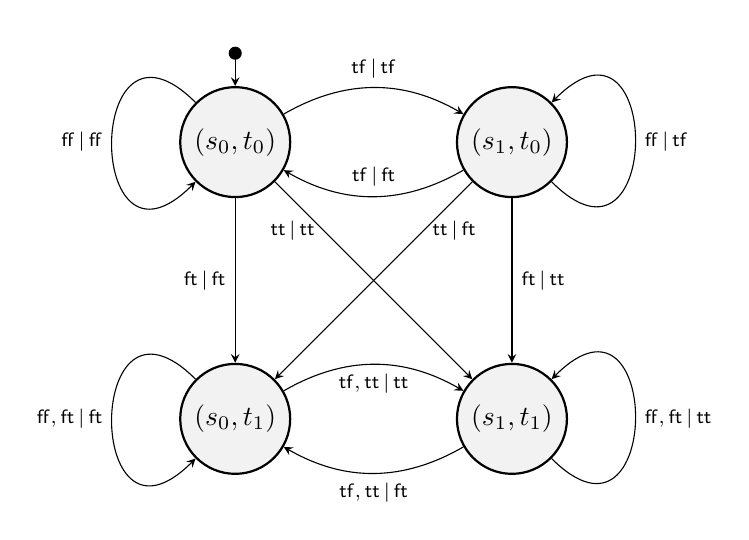
\begin{tikzpicture}[
        bezier bounding box=true,
        ->,
        >=stealth,
        node distance=0.25cm,
        every node/.style={font=\scriptsize},
        every state/.style={font=\normalsize, thick, fill=gray!10},
        initial text=$ $,
        initial distance=0.5cm,
        every initial by arrow/.style={*->},
        x=20pt,
        y=20pt
    ]
    \node[state, initial above] (s0) at (0,0) {\((s_0,t_0)\)};
    \node[state] (s1) at (5,0) {\((s_1,t_0)\)};
    \node[state] (s2) at (0,-5) {\((s_0,t_1)\)};
    \node[state] (s3) at (5,-5) {\((s_1,t_1)\)};

    \draw (s0) edge[out=135, in=225, loop, distance=2cm] node[left]{
            \(\trs{\mathsf{ff}}{\mathsf{ff}}\)
        } (s0);
    \draw (s0) edge[left] node{\(\trs{\mathsf{ft}}{\mathsf{ft}}\)} (s2);
    \draw (s0) edge[bend left, above] node{\(\trs{\mathsf{tf}}{\mathsf{tf}}\)} (s1);
    \draw (s0) edge[left, near start] node{\(\trs{\mathsf{tt}}{\mathsf{tt}}\)} (s3);

    \draw (s1) edge[out=315, in=45, loop, distance=2cm] node[right]{
            \(\trs{\mathsf{ff}}{\mathsf{tf}}\)
        } (s1);
    \draw (s1) edge[bend left, above] node{\(\trs{\mathsf{tf}}{\mathsf{ft}}\)} (s0);
    \draw (s1) edge[right] node{\(\trs{\mathsf{ft}}{\mathsf{tt}}\)} (s3);
    \draw (s1) edge[right, near start] node{\(\trs{\mathsf{tt}}{\mathsf{ft}}\)} (s2);

    \draw (s2) edge[out=135, in=225, loop, distance=2cm] node[left]{
            \(\trs{\mathsf{ff},\mathsf{ft}}{\mathsf{ft}}\)
        } (s2);
    \draw (s2) edge[bend left, below] node{\(\trs{\mathsf{tf},\mathsf{tt}}{\mathsf{tt}}\)} (s3);

    \draw (s3) edge[out=315, in=45, loop, distance=2cm] node[right]{
            \(\trs{\mathsf{ff},\mathsf{ft}}{\mathsf{tt}}\)
        } (s3);
    \draw (s3) edge[bend left, below] node{\(\trs{\mathsf{tf},\mathsf{tt}}{\mathsf{ft}}\)} (s2);
\end{tikzpicture}
\end{document}